\section{Yields and distributions}

In this section we summarize the status of the analysis after selection, showing the inputs to the final results, namely the event yields and errors in the full signal region and in a restricted  $\mllll$ range, and the distributions of the main kinematic variables in data and MC. 

\subsection{Signal Region Yields}

The number of candidates observed in data and the expected yields for the backgrounds and Higgs boson signal after the full event selection are reported in Table~\ref{tab:EventYieldsFull} for the full range of $\mllll$ and in Table~\ref{tab:EventYieldsPeak} for a $118<\mllll<130~\GeV$ mass window around the Higgs boson peak.
%in Table~\ref{tab:EventYieldsPeak} for a $118<\mllll<130~\GeV$ mass window around the Higgs boson peak, 
Table~\ref{tab:EventYieldsPeakCateg} shows the expected and observed yields for each of the 22 event categories.

%============
\begin{table}[htb]
	\begin{center}
		\small
		\caption{The number of expected background and signal events 
			and number observed candidates after full analysis selection, for each final state, 
			for the full mass range $\mllll>70~\GeV$, for an integrated luminosity of $\usedLumiC$.
			Signal and ZZ backgrounds are estimated from Monte Carlo simulation,
			$\cPZ$+X is estimated from data.
			\label{tab:EventYieldsFull}}
			\begin{tabular}{l|c|c|c|c}
	\hline
	\hline
	\textbf{Channel} & $4\Pe$ & $4\Pgm$ & $2\Pe2\Pgm$ & $4\ell$ \\
	\hline
	\qqZZ & $333.01^{+ y.y}_{- z.z}$ & $622.20^{+ y.y}_{- z.z}$ & $815.20^{+ y.y}_{- z.z}$ & $1770.41^{+ y.y}_{- z.z}$ \\
	\ggZZ & $75.11^{+ y.y}_{- z.z}$ & $116.55^{+ y.y}_{- z.z}$ & $176.86^{+ y.y}_{- z.z}$ & $368.52^{+ y.y}_{- z.z}$ \\
	\cPZ\ + X & $19.37^{+ y.y}_{- z.z}$ & $50.75^{+ y.y}_{- z.z}$ & $64.84^{+ y.y}_{- z.z}$ & $134.96^{+ y.y}_{- z.z}$ \\
	\hline
	Sum of backgrounds & $427.50^{+ y.y}_{- z.z}$ & $789.50^{+ y.y}_{- z.z}$ & $1056.89^{+ y.y}_{- z.z}$ & $2273.89^{+ y.y}_{- z.z}$ \\
	\hline
	Signal ($\mH=125~\GeV$) & $19.58^{+ y.y}_{- z.z}$ & $40.83^{+ y.y}_{- z.z}$ & $50.68^{+ y.y}_{- z.z}$ & $111.09^{+ y.y}_{- z.z}$ \\
	\hline
	Total expected & $447.08^{+ y.y}_{- z.z}$ & $830.33^{+ y.y}_{- z.z}$ & $1107.57^{+ y.y}_{- z.z}$ & $2384.98^{+ y.y}_{- z.z}$ \\
	\hline
	Observed & 462 & 850 & 1130 & 2442 \\
	\hline
	\hline
\end{tabular}

	%		\begin{tabular}{l|c|c|c|c}
%				\hline
		%		\hline
			%	\textbf{Channel} & $4\Pe$ & $4\Pgm$ & $2\Pe2\Pgm$ & $4\ell$ \\
				%\hline
				%\qqZZ & $368.00^{+ y.y}_{- z.z}$ & $646.66^{+ y.y}_{- z.z}$ & $871.70^{+ y.y}_{- z.z}$ & $1886.35^{+ y.y}_{- z.z}$ \\
				%\ggZZ & $82.36^{+ y.y}_{- z.z}$ & $122.98^{+ y.y}_{- z.z}$ & $190.37^{+ y.y}_{- z.z}$ & $395.71^{+ y.y}_{- z.z}$ \\
				%\cPZ\ + X & $22.27^{+ y.y}_{- z.z}$ & $51.41^{+ y.y}_{- z.z}$ & $63.90^{+ y.y}_{- z.z}$ & $137.58^{+ y.y}_{- z.z}$ \\
				%\hline
				%Sum of backgrounds & $472.63^{+ y.y}_{- z.z}$ & $821.05^{+ y.y}_{- z.z}$ & $1125.97^{+ y.y}_{- z.z}$ & $2419.65^{+ y.y}_{- z.z}$ \\
				%\hline
				%Signal ($\mH=125~\GeV$) & $21.68^{+ y.y}_{- z.z}$ & $42.57^{+ y.y}_{- z.z}$ & $54.32^{+ y.y}_{- z.z}$ & $118.57^{+ y.y}_{- z.z}$ \\
				%\hline
				%Total expected & $494.31^{+ y.y}_{- z.z}$ & $863.61^{+ y.y}_{- z.z}$ & $1180.29^{+ y.y}_{- z.z}$ & $2538.22^{+ y.y}_{- z.z}$ \\
				%\hline
				%Observed & 466 & 845 & 1121 & 2432\\
				%\hline
				%\hline
			%\end{tabular}
	\end{center}
\end{table}
%============


\begin{table}[htb]
	\begin{center}
		\small
		\caption{The number of expected background and signal events and number of observed candidates after full analysis selection, for each event category, for the mass range $118<\mllll<130~\GeV$, for an integrated luminosity of $\usedLumiC$.
			The yields are given for the different production modes.
			Signal and ZZ backgrounds are estimated from Monte Carlo simulation, 
			$\cPZ$+X is estimated from data.
			\label{tab:EventYieldsPeak}}
		%\resizebox{\textwidth}{!}
		{
		%	\begin{tabular}{l|c|c|c|c}
			\begin{tabular}{l|c|c|c}
				\hline
				\hline
%				\textbf{Channel} & $4\Pe$ & $4\Pgm$ & $2\Pe2\Pgm$ & $4\ell$ \\
				\textbf{Channel} & $4\Pgm$ & $4\Pe$ & $2\Pe2\Pgm$  \\
				\hline
				Signal ($m_{H}$ =125 GeV)  &37.09  &16.35  &44.16   \\
				 qqZZ     &14.10  &5.33   &16.43   \\
				 ggZZ     &1.30   &0.63   &1.15    \\
				 ZX       &6.53   &1.72   &7.22    \\
				 Total expected   &59.02 &24.03  &68.96   \\
				 Data     &50     &23     &63      \\
				%\qqZZ & $5.77^{+ y.y}_{- z.z}$ & $15.49^{+ y.y}_{- z.z}$ & $17.78^{+ y.y}_{- z.z}$ & $39.04^{+ y.y}_{- z.z}$ \\
				%\ggZZ & $0.71^{+ y.y}_{- z.z}$ & $1.54^{+ y.y}_{- z.z}$ & $1.35^{+ y.y}_{- z.z}$ & $3.60^{+ y.y}_{- z.z}$ \\
				%\cPZ\ + X & $2.04^{+ y.y}_{- z.z}$ & $7.03^{+ y.y}_{- z.z}$ & $7.34^{+ y.y}_{- z.z}$ & $16.41^{+ y.y}_{- z.z}$ \\
				%\hline
				%Sum of backgrounds & $8.52^{+ y.y}_{- z.z}$ & $24.07^{+ y.y}_{- z.z}$ & $26.47^{+ y.y}_{- z.z}$ & $59.05^{+ y.y}_{- z.z}$ \\
				%\hline
				%Signal ($\mH=125~\GeV$) & $18.32^{+ y.y}_{- z.z}$ & $38.68^{+ y.y}_{- z.z}$ & $47.67^{+ y.y}_{- z.z}$ & $104.68^{+ y.y}_{- z.z}$ \\
				%\hline
				%Total expected & $26.84^{+ y.y}_{- z.z}$ & $62.75^{+ y.y}_{- z.z}$ & $74.14^{+ y.y}_{- z.z}$ & $163.73^{+ y.y}_{- z.z}$ \\
				%\hline
				%Observed & 22 & 50 & 61 & 133 \\
				\hline
				\hline
		\end{tabular}}
	\end{center}
\end{table}


\begin{table}[htb]
	\begin{center}
		\small
		\caption{The number of expected background and signal events and number of observed candidates after full analysis selection, for each event category, for the mass range $118<\mllll<130~\GeV$, for an integrated luminosity of \usedLumiABC.
			The yields are given for the different production modes.
			Signal and ZZ backgrounds are estimated from Monte Carlo simulation, 
			$\cPZ$+X is estimated from data.
			\label{tab:EventYieldsPeakCateg}}
		\resizebox{\textwidth}{!}
		{
		%	\begin{tabular}{c|cccccccccc|ccc|c|c}
				\begin{tabular}{cccccccc|ccc|cc|c}
				\hline
				\hline
				Event & \multicolumn{7}{c|}{Signal} & \multicolumn{3}{c|}{Background} &  \multicolumn{2}{c|}{Expected} & Observed \\
				category             & $\ggH$ &VBF    &WH    &ZH    &ttH   &bbH   &tqH   &$\qqZZ$  &$\ggZZ$   &$\cPZ$ + X  &signal&total& \\
				\hline
				ggH-0j/pT[0,10]      &25.31  &0.08  &0.02  &0.02  &0.00  &0.14  &0.00  &26.46  &0.97  &1.19    &25.57  &54.18   &61.00   \\
				ggH-0j/pT[10-200]    &86.80  &1.69  &0.54  &0.86  &0.00  &0.90  &0.00  &35.42  &3.79  &15.48   &90.80  &145.49  &153.00  \\
				ggH-1j/pT[0-60]      &26.24  &1.43  &0.50  &0.45  &0.01  &0.43  &0.01  &10.26  &1.19  &5.54    &29.06  &46.05   &40.00   \\
				ggH-1j/pT[60-120]    &12.35  &1.24  &0.45  &0.47  &0.01  &0.10  &0.01  &2.76   &0.16  &3.21    &14.63  &20.76   &17.00   \\
				ggH-1j/pT[120-200]   &3.31   &0.62  &0.17  &0.26  &0.00  &0.02  &0.00  &0.38   &0.00  &0.52    &4.38   &5.28    &6.00    \\
				ggH-2j/pT[0-60]      &3.68   &0.29  &0.14  &0.14  &0.06  &0.09  &0.02  &0.97   &0.15  &2.07    &4.42   &7.60    &9.00    \\
				ggH-2j/pT[60-120]    &5.17   &0.54  &0.22  &0.22  &0.09  &0.04  &0.02  &0.84   &0.07  &1.86    &6.30   &9.06    &12.00   \\
				ggH-2j/pT[120-200]   &2.90   &0.40  &0.15  &0.17  &0.07  &0.01  &0.02  &0.26   &0.00  &0.40    &3.71   &4.37    &5.00    \\
				ggH/pT$>$200         &2.72   &0.65  &0.21  &0.24  &0.06  &0.01  &0.02  &0.16   &0.00  &0.21    &3.91   &4.28    &2.00    \\
				ggH-2j/mJJ$>$350     &0.82   &0.17  &0.06  &0.05  &0.04  &0.01  &0.01  &0.16   &0.02  &0.65    &1.16   &1.98    &3.00    \\
				VBF-1j               &14.17  &2.94  &0.20  &0.18  &0.00  &0.12  &0.01  &2.37   &0.43  &1.05    &17.61  &21.46   &20.00   \\
				VBF-2j/mJJ[350,700]  &0.80   &1.11  &0.01  &0.01  &0.00  &0.01  &0.00  &0.08   &0.02  &0.04    &1.95   &2.09    &2.00    \\
				VBF-2j/mJJ$>$700     &0.43   &1.80  &0.00  &0.00  &0.00  &0.00  &0.00  &0.02   &0.01  &0.03    &2.25   &2.31    &2.00    \\
				VBF-3j/mJJ$>$350     &2.43   &2.15  &0.06  &0.07  &0.02  &0.03  &0.05  &0.24   &0.06  &0.96    &4.81   &6.07    &6.00    \\
				VBF-2j/pT$>$200      &0.42   &0.76  &0.01  &0.01  &0.01  &0.00  &0.01  &0.01   &0.00  &0.03    &1.22   &1.26    &0.00    \\
				VBF-rest             &2.40   &0.87  &0.11  &0.10  &0.03  &0.04  &0.01  &0.34   &0.06  &0.74    &3.56   &4.70    &2.00    \\
				VH-lep/pTV[0-150]    &0.24   &0.04  &0.71  &0.25  &0.08  &0.02  &0.02  &0.82   &0.14  &0.40    &1.37   &2.72    &5.00    \\
				VH-lep/pTV$>$150     &0.02   &0.01  &0.21  &0.08  &0.04  &0.00  &0.01  &0.01   &0.00  &0.02    &0.36   &0.40    &0.00    \\
				VH-had/mJJ[60-120]   &4.11   &0.25  &1.01  &1.20  &0.11  &0.07  &0.02  &0.70   &0.05  &1.36    &6.77   &8.89    &8.00    \\
				VH-rest              &0.56   &0.04  &0.08  &0.07  &0.03  &0.00  &0.00  &0.08   &0.00  &0.15    &0.77   &1.01    &1.00    \\
				ttH-had              &0.19   &0.05  &0.03  &0.06  &0.82  &0.01  &0.03  &0.01   &0.00  &0.45    &1.19   &1.66    &2.00    \\
				ttH-lep              &0.02   &0.00  &0.02  &0.02  &0.60  &0.00  &0.03  &0.03   &0.00  &0.12    &0.70   &0.85    &0.00    \\
				\hline
				\hline
		\end{tabular}}
	\end{center}
\end{table}

\subsection{Signal Region Distributions}

The reconstructed four-lepton invariant mass distribution is shown in Figure~\ref{fig:Mass4lC} for the full dataset, and compared to expectations from the SM backgrounds, first for the full mass range, and then zooming on the low-mass range and high-mass range. 
In Figure~\ref{fig:Mass4l-2C}, the same distributions are shown split by final state ($4e$, $4\mu$, and $2e2\mu$), for the two same mass ranges.
In Figure~\ref{fig:Mass4l-3C}, they are split by event category, for the low-mass range.
The SM background distributions are obtained combining the rate normalization from data-driven methods and knowledge on shapes taken from the MC samples. \\
%\textbf{FIXME: 2016 MC is used.} \\
%\textbf{Z+X estimation is scaled from 2016.}.\\
%\textbf{(low mass) Signal region is Blinded, as well as high mass points} \\

%=============
\begin{figure}[!htb]
	\vspace*{0.3cm}
	\begin{center}
		
\includegraphics[width=0.85\textwidth]{Figures/KinDistr/2018/M4lMain_Unblinded_4l_Inclusive.pdf} \\ %a_M4l_Full_4l_inclusive_.pdf}\\
		
\includegraphics[width=0.45\textwidth]{Figures/KinDistr/2018/M4lMainZoomed_Unblinded_4l_Inclusive.pdf} %a_M4l_70170_4l_inclusive_.pdf}
		
\includegraphics[width=0.45\textwidth]{Figures/KinDistr/2018/M4lMainHighMass_Unblinded_4l_Inclusive.pdf} %a_M4l_above170_4l_inclusive_.pdf}
		\caption{Distribution of the four-lepton reconstructed invariant mass $\mllll$ in the full mass range (top) and the low-mass range (bottom left) and high-mass range (bottom right). Points with error bars represent the data and stacked histograms represent expected distributions. The $125~\GeV$ Higgs boson signal and the $\cPZ\cPZ$ backgrounds are normalized to the SM expectation, the $\cPZ$+X background to the estimation from data.
			%what about high mass range??
			%No event is observed with $\mllll>1\TeV$.
			\label{fig:Mass4lC}}
	\end{center}
\end{figure}
%=======

%=============
\begin{figure}[!htb]
	\vspace*{0.3cm}
	\begin{center}
		
\includegraphics[width=0.56\textwidth]{Figures/KinDistr/2018/M4lMain_Unblinded_4e_Inclusive.pdf}
		
\includegraphics[width=0.43\textwidth]{Figures/KinDistr/2018/M4lMainZoomed_Unblinded_4e_Inclusive.pdf}\\
		
\includegraphics[width=0.56\textwidth]{Figures/KinDistr/2018/M4lMain_Unblinded_4mu_Inclusive.pdf}
		
\includegraphics[width=0.43\textwidth]{Figures/KinDistr/2018/M4lMainZoomed_Unblinded_4mu_Inclusive.pdf}\\
		
\includegraphics[width=0.56\textwidth]{Figures/KinDistr/2018/M4lMain_Unblinded_2e2mu_Inclusive.pdf}
		
\includegraphics[width=0.43\textwidth]{Figures/KinDistr/2018/M4lMainZoomed_Unblinded_2e2mu_Inclusive.pdf}\\
		\caption{ Distribution of the four-lepton reconstructed mass in several sub-channels: $4e$ (top), $4\mu$ (middle), $2e2\mu$ for the low-mass range (bottom) for the full mass range (left) and the low-mass range (right).
			\label{fig:Mass4l-2C}}
	\end{center}
\end{figure}
%==================

%=============
\begin{figure}[!htb]
	\vspace*{0.3cm}
	\begin{center}
		\subfigure[]{ 
\includegraphics[width=0.45\textwidth]{Figures/KinDistr/2018/M4lMain_Unblinded_4l_UnTagged.pdf}} 
		\subfigure[]{ 
\includegraphics[width=0.45\textwidth]{Figures/KinDistr/2018/M4lMain_Unblinded_4l_VBF1jTagged.pdf}} \\
		\subfigure[]{ 
\includegraphics[width=0.45\textwidth]{Figures/KinDistr/2018/M4lMain_Unblinded_4l_VBF2jTagged.pdf}} 
		\subfigure[]{ 
\includegraphics[width=0.45\textwidth]{Figures/KinDistr/2018/M4lMain_Unblinded_4l_VHHadrTagged.pdf}} \\
		\subfigure[]{ 
\includegraphics[width=0.33\textwidth]{Figures/KinDistr/2018/M4lMain_Unblinded_4l_VHLeptTagged.pdf}} 
		%\subfigure[]{ 
\includegraphics[width=0.33\textwidth]{Figures/KinDistr/M4lMain_Blinded_4l_VHMETTagged.pdf}} \\
		\subfigure[]{ 
\includegraphics[width=0.33\textwidth]{Figures/KinDistr/2018/M4lMain_Unblinded_4l_ttHHadrTagged.pdf}} 
		\subfigure[]{ 
\includegraphics[width=0.33\textwidth]{Figures/KinDistr/2018/M4lMain_Unblinded_4l_ttHLeptTagged.pdf}} \\
		\caption{ Distribution of the four-lepton reconstructed mass in the seven event categories for the low-mass range.
			(a) untagged category (b) VBF-1jet-tagged category (c) VBF-2jet-tagged category (d) VH-hadronic-tagged category (e) VH-leptonic-tagged category (f) \ttH-hadronic-tagged category (g) \ttH-leptonic-tagged category.
			%(f) VH-MET-tagged category (g) \ttH-hadronic-tagged category (h) \ttH-leptonic-tagged category.
			\label{fig:Mass4l-3C}}
	\end{center}
\end{figure}
%=======


The reconstructed dilepton invariant masses selected as Z$_1$ and Z$_2$ are shown in Figures~\ref{fig:MZ1C} together with their correlation, both full range of of $\mllll$ and focusing on a $118<\mllll<130~\GeV$ mass window around the Higgs boson peak.
%and~\ref{fig:MZ2} in the full mass range.
%with their correlation, both in the full range of $\mllll$ and focusing on a $118<\mllll<130~\GeV$ mass window around the Higgs boson peak.
Similarly, the decay discriminant $\KD$, $\DbkgVBFdec$ and $\DbkgVHdec$ are shown in Fig.~\ref{fig:KDvsM4lC},~\ref{fig:KDVBFsvsM4lC} and~\ref{fig:KDVHsvsM4lC} in this window. % in these two windows, as well as its correlation with the four-lepton invariant mass.
The four production mechanism discriminant $\DMeVbfjj$, $\DMeVbfj$, $\DMeWh$, and $\DMeZh$ are shown in Fig.~\ref{fig:DprodC} in the $118<\mllll<130~\GeV$ mass window, for events with at least two selected jets (except $\DMeVbfj$ which is for events with exactly one selected jet). 
Their correlations with $\mllll$ are shown in Fig.~\ref{fig:Dprod-corrC}. 

%=============
\begin{figure}[!htb]
	\vspace*{0.3cm}
	\begin{center}
		%
\includegraphics[width=0.450\textwidth]{Figures/KinDistr/2018/MZ1_Unblinded_4l_Inclusive.pdf} %fb_MZ1_4l_inclusive_.pdf}
		
\includegraphics[width=0.450\textwidth]{Figures/KinDistr/2018/MZ1_M4L118130_Unblinded_4l_Inclusive.pdf} \\ %fb_MZ1_4l_inclusive_.pdf}
		%
\includegraphics[width=0.450\textwidth]{Figures/KinDistr/2018/MZ2_Unblinded_4l_Inclusive.pdf} %fb_MZ1_4l_inclusive_.pdf}
		
\includegraphics[width=0.450\textwidth]{Figures/KinDistr/2018/MZ2_M4L118130_Unblinded_4l_Inclusive.pdf} \\ %fb_MZ1_4l_inclusive_.pdf}
		%
\includegraphics[width=0.45\textwidth]{Figures/KinDistr/2018/MZ1vsMZ2_Unblinded_Inclusive.pdf}
		
\includegraphics[width=0.45\textwidth]{Figures/KinDistr/2018/MZ1vsMZ2_M4L118130_Unblinded_Inclusive.pdf}
		\caption{%\textb{FIXME: Add low mass plots after unblinding.}
			Distribution of the $\cPZ_1$ (top), $\cPZ_2$ (middle) and $\cPZ_1$ vs $\cPZ_2$ (bottom) reconstructed invariant masses for the full mass range (left) and the low mass ($118<\mllll<130~\GeV$) range (right). 
			%Distribution of the $\cPZ_1$  reconstructed invariant masses for the full mass range (blinded), for all final states (top left), and for 4e (top right), 4mu (bottom left) and 2e2mu (bottom right) separately. 
			The stacked histograms and the gray scale represent expected distributions, and points represent the data. The $125~\GeV$ Higgs boson signal and the $\cPZ\cPZ$ backgrounds are normalized to the SM expectation, the $\cPZ$+X background to the estimation from data.
			%Distribution of the $\cPZ_1$ (left) and $\cPZ_2$ (center) reconstructed invariant masses and correlation between the two (right), for the full mass range (top row) and the mass region $118<\mllll<130~\GeV$ (bottom row). The stacked histograms and the gray scale represent expected distributions, and points represent the data. The $125~\GeV$ Higgs boson signal and the $\cPZ\cPZ$ backgrounds are normalized to the SM expectation, the $\cPZ$+X background to the estimation from data.
			\label{fig:MZ1C}}
	\end{center}
\end{figure}
%=======


%=======
\begin{figure}[!htb]
	\vspace*{0.3cm}
	\begin{center}
	  
\includegraphics[width=0.455\textwidth]{Figures/KinDistr/2018/KD_Unblinded_4l_Inclusive.pdf} %d_KD_4l_inclusive_.pdf}KD_Blinded_4l_Inclusive.pdf
		
\includegraphics[width=0.455\textwidth]{Figures/KinDistr/2018/KD_M4L118130_Unblinded_4l_Inclusive.pdf} \\
		%
\includegraphics[width=0.455\textwidth]{Figures/KinDistr/2018/KDvsM4l_Unblinded_Inclusive.pdf}
		
\includegraphics[width=0.455\textwidth]{Figures/KinDistr/2018/KDvsM4lZoomed_Unblinded_all_categories.pdf} 
                
\includegraphics[width=0.455\textwidth]{Figures/KinDistr/2018/KDvsM4lHighMass_Unblinded_Inclusive.pdf} \\
		
		%\caption{\textb{FIXME: Add low mass plots after unblinding.}
			%One-dimensional distribution of the kinematic discriminant $\KD$ in the full mass range (blinded), for all final states (top left) and for 4e  (top right), 4mu (bottom left) and 2e2mu (bottom right) separately.  Points with error bars represent the data and stacked histograms represent expected distributions. The $125~\GeV$ Higgs boson signal and the $\cPZ\cPZ$ backgrounds are normalized to the SM expectation, the $\cPZ$+X background to the estimation from data.
			Top row: One-dimensional distribution of the kinematic discriminant $\KD$ in the full mass range (left) and in the mass region $118<\mllll<130~\GeV$ (right). Points with error bars represent the data and stacked histograms represent expected distributions. The $125~\GeV$ Higgs boson signal and the $\cPZ\cPZ$ backgrounds are normalized to the SM expectation, the $\cPZ$+X background to the estimation from data.
			Bottom row: Distribution of the kinematic discriminant $\KD$ versus the four-lepton reconstructed mass $\mllll$ in the low-mass region (left) and in the high-mass region (right). The gray scale represents the expected relative density of $\cPZ\cPZ$ background plus Higgs boson signal for $\mH=125~\GeV$. The points show the data and the horizontal bars represent the measured mass uncertainties. 
			\label{fig:KDvsM4lC}}
	\end{center}
\end{figure}
%=======

%=======
\begin{figure}[!htb]
	\vspace*{0.3cm}
	\begin{center}
		
\includegraphics[width=0.455\textwidth]{Figures/KinDistr/2018/DVBFDEC_Unblinded_4l_VBF2jTagged.pdf} %d_KD_4l_inclusive_.pdf}KD_Blinded_4l_Inclusive.pdf
		
\includegraphics[width=0.455\textwidth]{Figures/KinDistr/2018/DVBFDEC_M4L118130_Unblinded_4l_VBF2jTagged.pdf} \\
		
\includegraphics[width=0.455\textwidth]{Figures/KinDistr/2018/DVBFDECvsM4lZoomed_Unblinded_all_categories.pdf}
		%
\includegraphics[width=0.455\textwidth]{Figures/KinDistr/KDvsM4lZoomed_Unblinded_all_categories.pdf} \\
		\caption{ %\textb{FIXME: Add low mass plots after unblinding.}
			%One-dimensional distribution of the kinematic discriminant $\KD$ in the full mass range (blinded), for all final states (top left) and for 4e  (top right), 4mu (bottom left) and 2e2mu (bottom right) separately.  Points with error bars represent the data and stacked histograms represent expected distributions. The $125~\GeV$ Higgs boson signal and the $\cPZ\cPZ$ backgrounds are normalized to the SM expectation, the $\cPZ$+X background to the estimation from data.
			Top row: One-dimensional distribution of the kinematic discriminant $\DbkgVBFdec$ in the full mass range (left) and in the mass region $118<\mllll<130~\GeV$ (right). Points with error bars represent the data and stacked histograms represent expected distributions. The $125~\GeV$ Higgs boson signal and the $\cPZ\cPZ$ backgrounds are normalized to the SM expectation, the $\cPZ$+X background to the estimation from data.
			Bottom row: Distribution of the kinematic discriminant $\DbkgVBFdec$ versus the four-lepton reconstructed mass $\mllll$ in the low-mass region.
			% (left) and in the high-mass region (right). 
			The gray scale represents the expected relative density of $\cPZ\cPZ$ background plus Higgs boson signal for $\mH=125~\GeV$. The points show the data and the horizontal bars represent the measured mass uncertainties. 
			\label{fig:KDVBFsvsM4lC}}
	\end{center}
\end{figure}
%=======

%=======
\begin{figure}[!htb]
	\vspace*{0.3cm}
	\begin{center}
	  
\includegraphics[width=0.455\textwidth]{Figures/KinDistr/2018/DVHDEC_Unblinded_4l_VHHadrTagged.pdf} 
		
\includegraphics[width=0.455\textwidth]{Figures/KinDistr/2018/DVHDEC_M4L118130_Unblinded_4l_VHHadrTagged.pdf} \\
		
\includegraphics[width=0.455\textwidth]{Figures/KinDistr/2018/DVHDECvsM4lZoomed_Unblinded_all_categories.pdf}
		%
\includegraphics[width=0.455\textwidth]{Figures/KinDistr/KDvsM4lZoomed_Unblinded_all_categories.pdf} \\
		\caption{ %\textb{FIXME: Add low mass plots after unblinding.}
			%One-dimensional distribution of the kinematic discriminant $\KD$ in the full mass range (blinded), for all final states (top left) and for 4e  (top right), 4mu (bottom left) and 2e2mu (bottom right) separately.  Points with error bars represent the data and stacked histograms represent expected distributions. The $125~\GeV$ Higgs boson signal and the $\cPZ\cPZ$ backgrounds are normalized to the SM expectation, the $\cPZ$+X background to the estimation from data.
			Top row: One-dimensional distribution of the kinematic discriminant $\DbkgVHdec$ in the full mass range (left) and in the mass region $118<\mllll<130~\GeV$ (right). Points with error bars represent the data and stacked histograms represent expected distributions. The $125~\GeV$ Higgs boson signal and the $\cPZ\cPZ$ backgrounds are normalized to the SM expectation, the $\cPZ$+X background to the estimation from data.
			Bottom row: Distribution of the kinematic discriminant $\DbkgVHdec$ versus the four-lepton reconstructed mass $\mllll$ in the low-mass region.
			% (left) and in the high-mass region (right). 
			The gray scale represents the expected relative density of $\cPZ\cPZ$ background plus Higgs boson signal for $\mH=125~\GeV$. The points show the data and the horizontal bars represent the measured mass uncertainties. 
			\label{fig:KDVHsvsM4lC}}
	\end{center}
\end{figure}
%=======

%=======
%\begin{figure}[!htb]
%\vspace*{0.3cm}
%\begin{center}
%
\includegraphics[width=0.75\textwidth]{Figures/KinDistr/KDvsM4lZoomed_Blinded_all_categories.pdf} %KD_Blinded_4l_Inclusive.pdf} %d_KD_4l_inclusive_.pdf}KD_Blinded_4l_Inclusive.pdf
%
\includegraphics[width=0.455\textwidth]{Figures/KinDistr/KD_Blinded_4e_Inclusive.pdf} \\
%
\includegraphics[width=0.455\textwidth]{Figures/KinDistr/KD_Blinded_4mu_Inclusive.pdf} 
%
\includegraphics[width=0.455\textwidth]{Figures/KinDistr/KD_Blinded_2e2mu_Inclusive.pdf} \\
%\includegraphics[width=0.45\textwidth]{Figures/KinDistr/d_KD_M4L118130_4l_inclusive_.pdf}\\
%\includegraphics[width=0.45\textwidth]{Figures/KinDistr/d_2D_M4lVsKD_M4L100170_4l_.pdf}
%\includegraphics[width=0.45\textwidth]{Figures/KinDistr/d_2D_M4lVsKD_M4L1701000_4l_.pdf}
%\caption{
%One-dimensional distribution of the kinematic discriminant $\KD$ in the full mass range (blinded), for all final states (top left) and for 4e  (top right), 4mu (bottom left) and 2e2mu (bottom right) separately.  Points with error bars represent the data and stacked histograms represent expected distributions. The $125~\GeV$ Higgs boson signal and the $\cPZ\cPZ$ backgrounds are normalized to the SM expectation, the $\cPZ$+X background to the estimation from data.
%Top row: One-dimensional distribution of the kinematic discriminant $\KD$ in the full mass range (left) and in the mass region $118<\mllll<130~\GeV$ (right). Points with error bars represent the data and stacked histograms represent expected distributions. The $125~\GeV$ Higgs boson signal and the $\cPZ\cPZ$ backgrounds are normalized to the SM expectation, the $\cPZ$+X background to the estimation from data.
%Bottom row: 
%Distribution of the kinematic discriminant $\KD$ versus the four-lepton reconstructed mass $\mllll$ in the low-mass region 
%(left) and in the high-mass region (right). 
%The gray scale represents the expected relative density of $\cPZ\cPZ$ background plus Higgs boson signal for $\mH=125~\GeV$. The points show the data and the horizontal bars represent the measured mass uncertainties. 
%\label{fig:KDvsM4l2}}
%\end{center}
%\end{figure}
%=======


%=======
\begin{figure}[!htb]
	\vspace*{0.3cm}
	\begin{center}
		
\includegraphics[width=0.45\textwidth]{Figures/KinDistr/2018/D1jet_M4L118130_Unblinded_4l_Inclusive.pdf}
		
\includegraphics[width=0.45\textwidth]{Figures/KinDistr/2018/D2jet_M4L118130_Unblinded_4l_Inclusive.pdf}\\
		
\includegraphics[width=0.45\textwidth]{Figures/KinDistr/2018/DVH_M4L118130_Unblinded_4l_Inclusive.pdf}
		%
\includegraphics[width=0.45\textwidth]{Figures/KinDistr/2018/DWH_M4L118130_Unblinded_4l_Inclusive.pdf} \\ %DWH_M4L118130_4l_inclusive_.pdf}
		%\includegraphics[width=0.45\textwidth]{Figures/KinDistr/e_DZH_M4L118130_4l_inclusive_.pdf}
		\caption{Distribution of the three production discriminants used for event categorization, in the mass region $118<\mllll<130~\GeV$. Points with error bars represent the data and stacked histograms represent expected distributions. The $125~\GeV$ Higgs boson signal and the $\cPZ\cPZ$ backgrounds are normalized to the SM expectation, the $\cPZ$+X background to the estimation from data. 
			\label{fig:DprodC}}
	\end{center}
\end{figure}
%=======

%=======
\begin{figure}[!htb]
	\vspace*{0.3cm}
	\begin{center}
		
\includegraphics[width=0.45\textwidth]{Figures/KinDistr/2018/D1jetvsM4lZoomed_Unblinded_Inclusive.pdf}
		
\includegraphics[width=0.45\textwidth]{Figures/KinDistr/2018/D2jetvsM4lZoomed_Unblinded_Inclusive.pdf}\\
		
\includegraphics[width=0.45\textwidth]{Figures/KinDistr/2018/DVHvsM4lZoomed_Unblinded_Inclusive.pdf}
		%\includegraphics[width=0.45\textwidth]{Figures/KinDistr/e_2D_M4lVsDWH_M4L100170_4l_.pdf}
		%\includegraphics[width=0.45\textwidth]{Figures/KinDistr/e_2D_M4lVsDZH_M4L100170_4l_.pdf}
		\caption{Distribution of the three production discriminants used for event categorization versus the four-lepton reconstructed mass $\mllll$ in the low-mass region. The gray scale represents the expected relative density of $\cPZ\cPZ$ background plus Higgs boson signal for $\mH=125~\GeV$. The points show the data and the horizontal bars represent the measured mass uncertainties.
			\label{fig:Dprod-corrC}}
	\end{center}
\end{figure}
%=======


\clearpage

The reconstructed four-lepton invariant mass distribution is shown for the full Run 2 in Fig.~\ref{fig:combination} for the sum of the  $4\Pe$, $4\Pgm$ and $2\Pe2\Pgm$ subchannels, and compared with the expectations from signal and background processes. 
% The normalization and shape of the Higgs boson signal and $\cPZ\cPZ$ backgrounds are obtained from simulation, while those of the $\cPZ$+X background are estimated from control samples in data, as described in Section~\ref{sec:redbkgd}. 
The error bars on the data points correspond to the so-called Garwood confidence intervals at 68\% confidence level (CL)~\cite{doi:GARWOOD}.
%The error bars on data points are asymmetric Poisson uncertainties that cover the 68\% probability interval around the central value~\cite{Cousins:1994yw}. 
  The observed distribution agrees with the expectation within the statistical uncertainties over the whole spectrum. The Fig.\ref{fig:STXS_Categorization} shows number of expected and observed events in all Stage 1.1 sub-categories for full Run 2.

%=============                                                                                                                    
\begin{figure}[!htb]
	\vspace*{0.3cm}
	\begin{center}	
		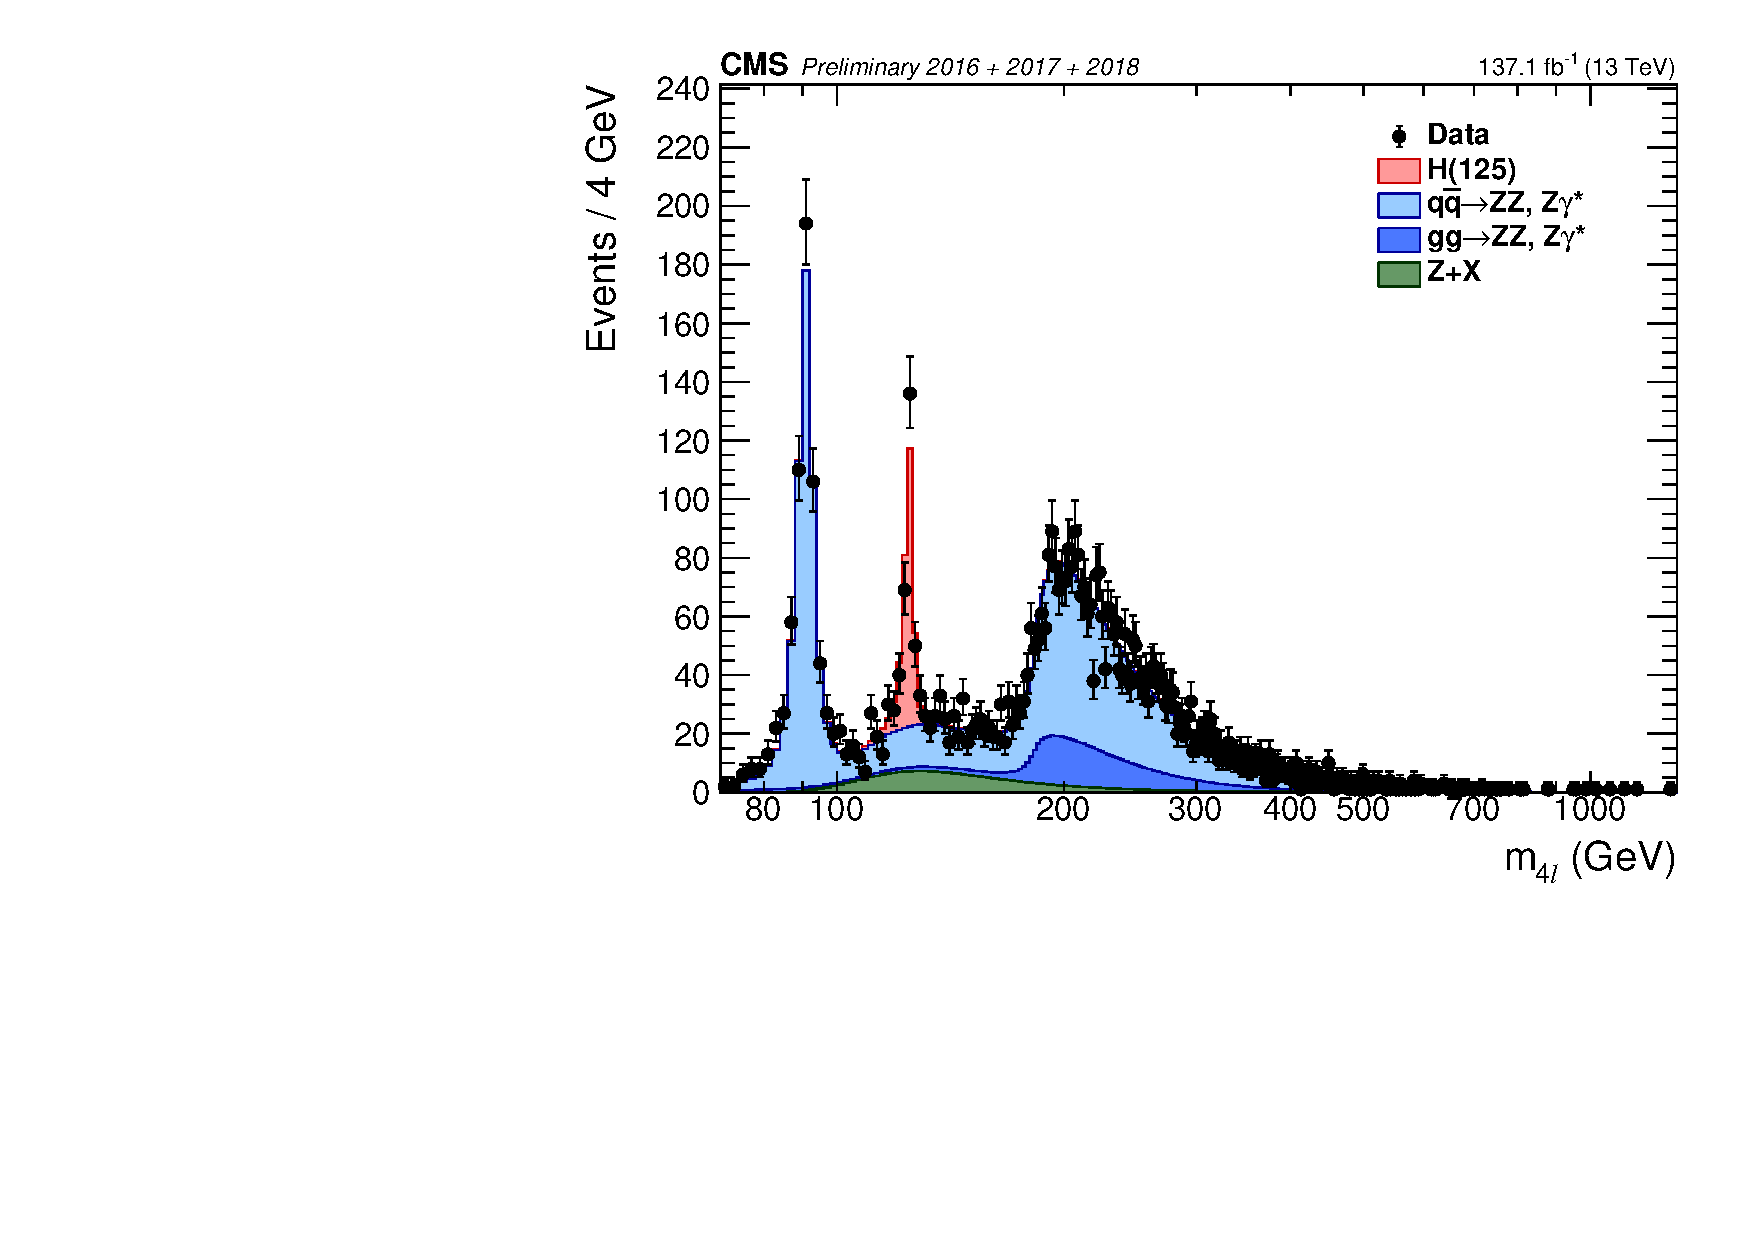
\includegraphics[width=0.6\textwidth]{Figures/KinDistr/2018/Combination.pdf} \\
		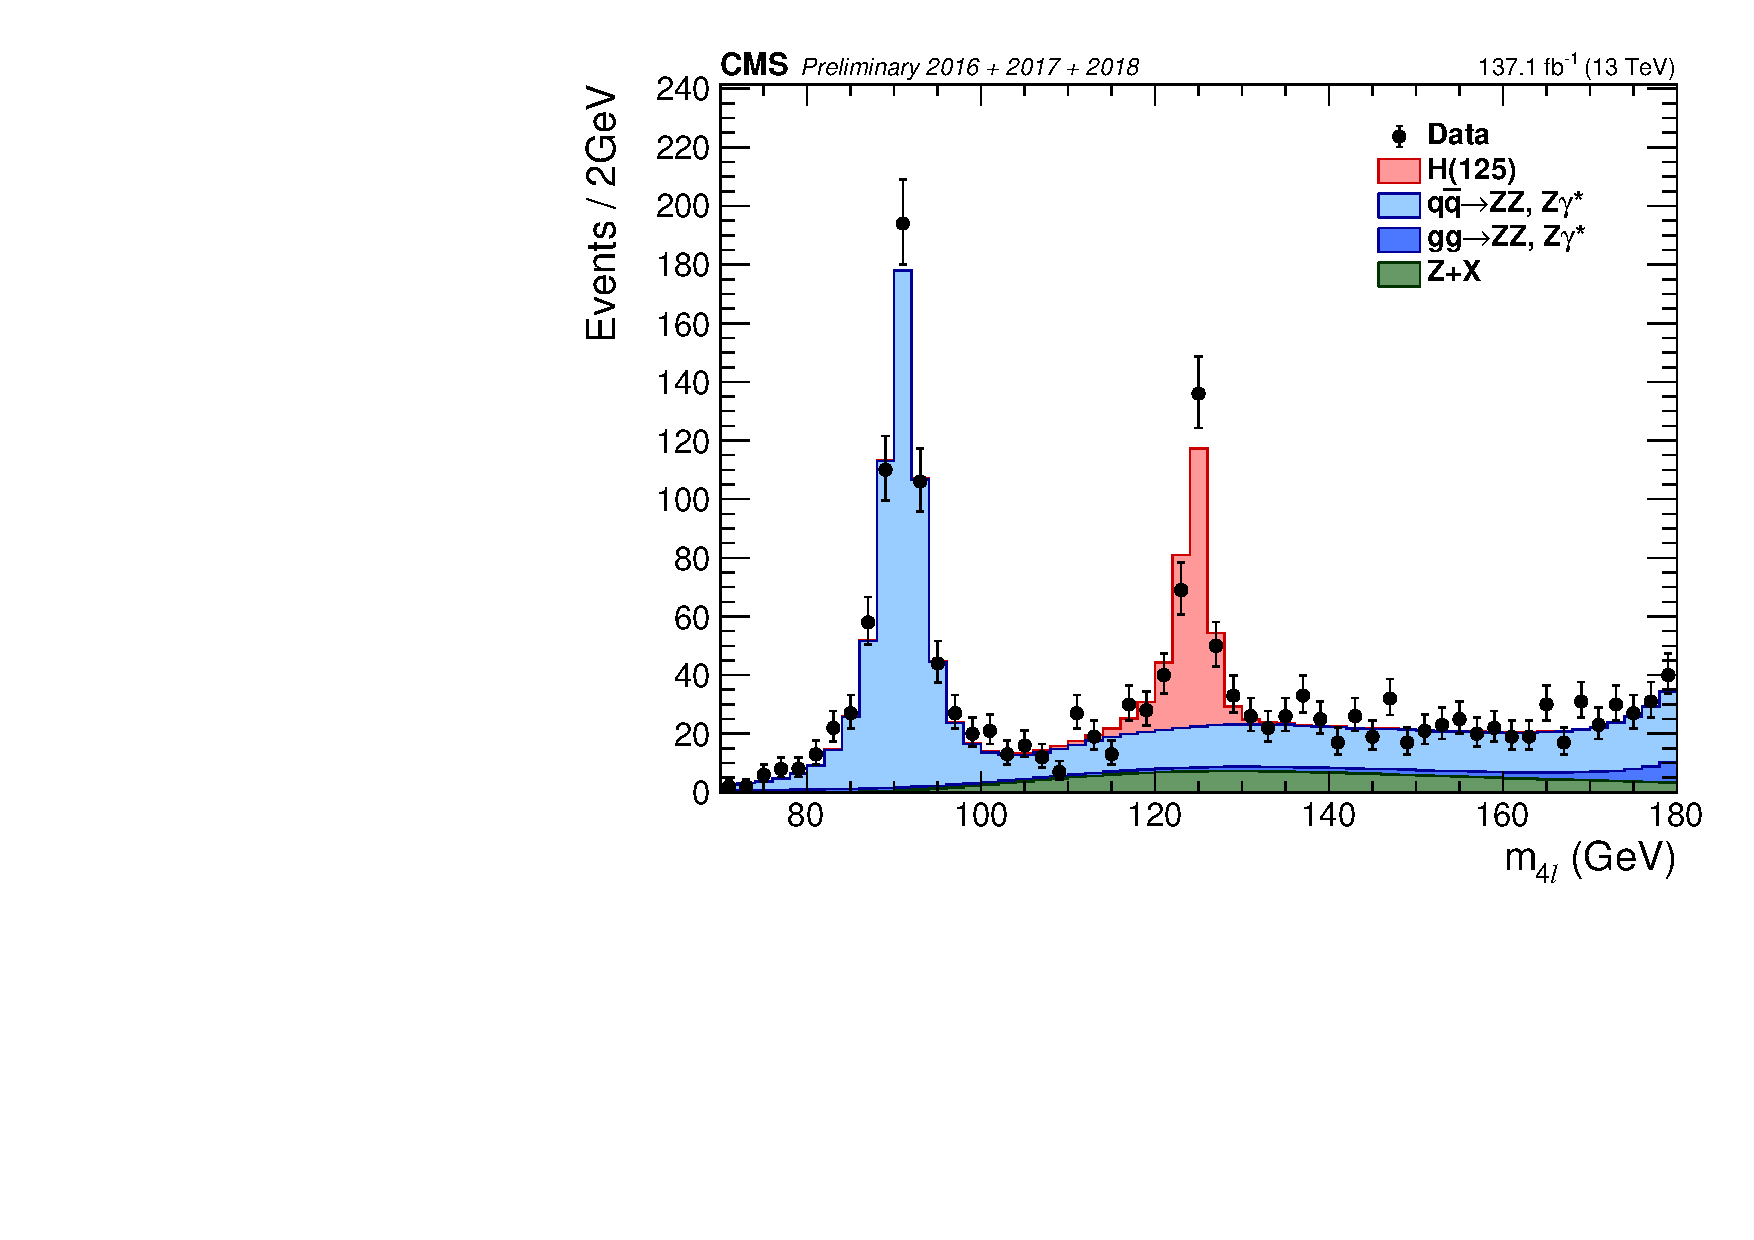
\includegraphics[width=0.6\textwidth]{Figures/KinDistr/2018/Combination_lowMass.pdf}
		\caption{Distribution of the reconstructed four-lepton invariant mass $\mllll$ up to $500\GeV$ (left) and the low-mass range (right), with Run 2 data. Points with error bars represent the data and stacked histograms represent expected distributions of the signal and background processes. The SM Higgs boson signal with $\mH=125\GeV$, denoted as ${\rm H}(125)$, and the $\cPZ\cPZ$ backgrounds are normalized to the SM expectation, the $\cPZ$+X background to the estimation from data. 
			%The order in perturbation theory used for the normalization of the irreducible backgrounds is described in Section~\ref{sec:irrbkgd}.
			\label{fig:combination}}
	\end{center}
\end{figure}
%=======        


%=============                                                                                                                    
\begin{figure}[!htb]
	\vspace*{0.3cm}
	\begin{center}	
		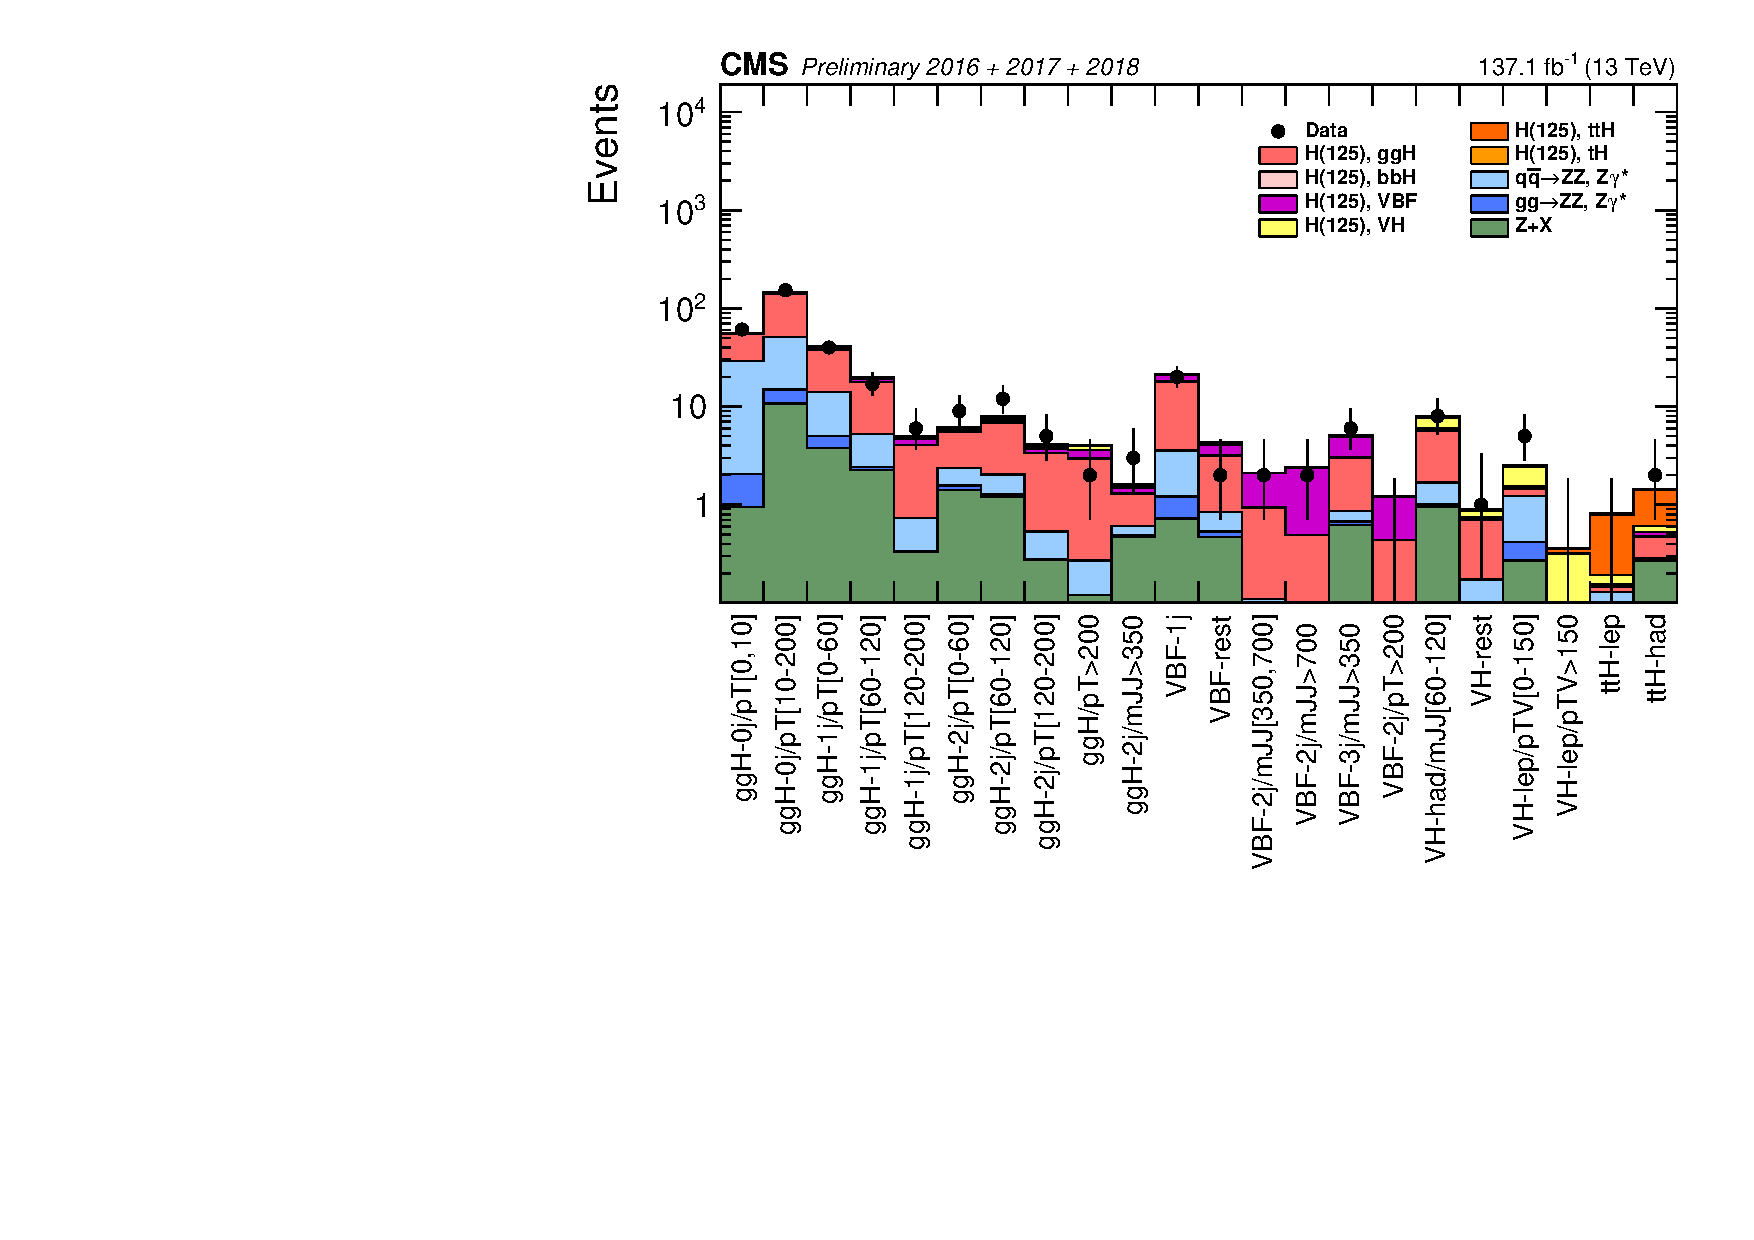
\includegraphics[width=0.9\textwidth]{Figures/KinDistr/2018/STXS_Categorization.pdf}
		\caption{Distributions of the expected and observed number of events for all Stage 1.1 sub-categories described in Section~\ref{subsec:STXS_Categories} in the mass region $118<\mllll<130\GeV$ with Run 2 data. Points with error bars represent the data and stacked histograms represent the expected numbers of the signal and background events. The different SM Higgs boson signal production modes with $\mH=125\GeV$, denoted as ${\rm H}(125)$, and the $\cPZ\cPZ$ backgrounds are normalized to the SM expectation, the $\cPZ$+X background to the estimation from data. 
			%The order in perturbation theory used for the normalization of the irreducible backgrounds is described in Section~\ref{sec:irrbkgd}.
			\label{fig:STXS_Categorization}}
	\end{center}
\end{figure}
%=======      
